\documentclass[tikz,border=7pt]{standalone}
\usepackage[T1]{fontenc}
\usepackage{lmodern}
\usetikzlibrary{arrows.meta,positioning,shapes.geometric,fit,backgrounds,calc}
\begin{document}
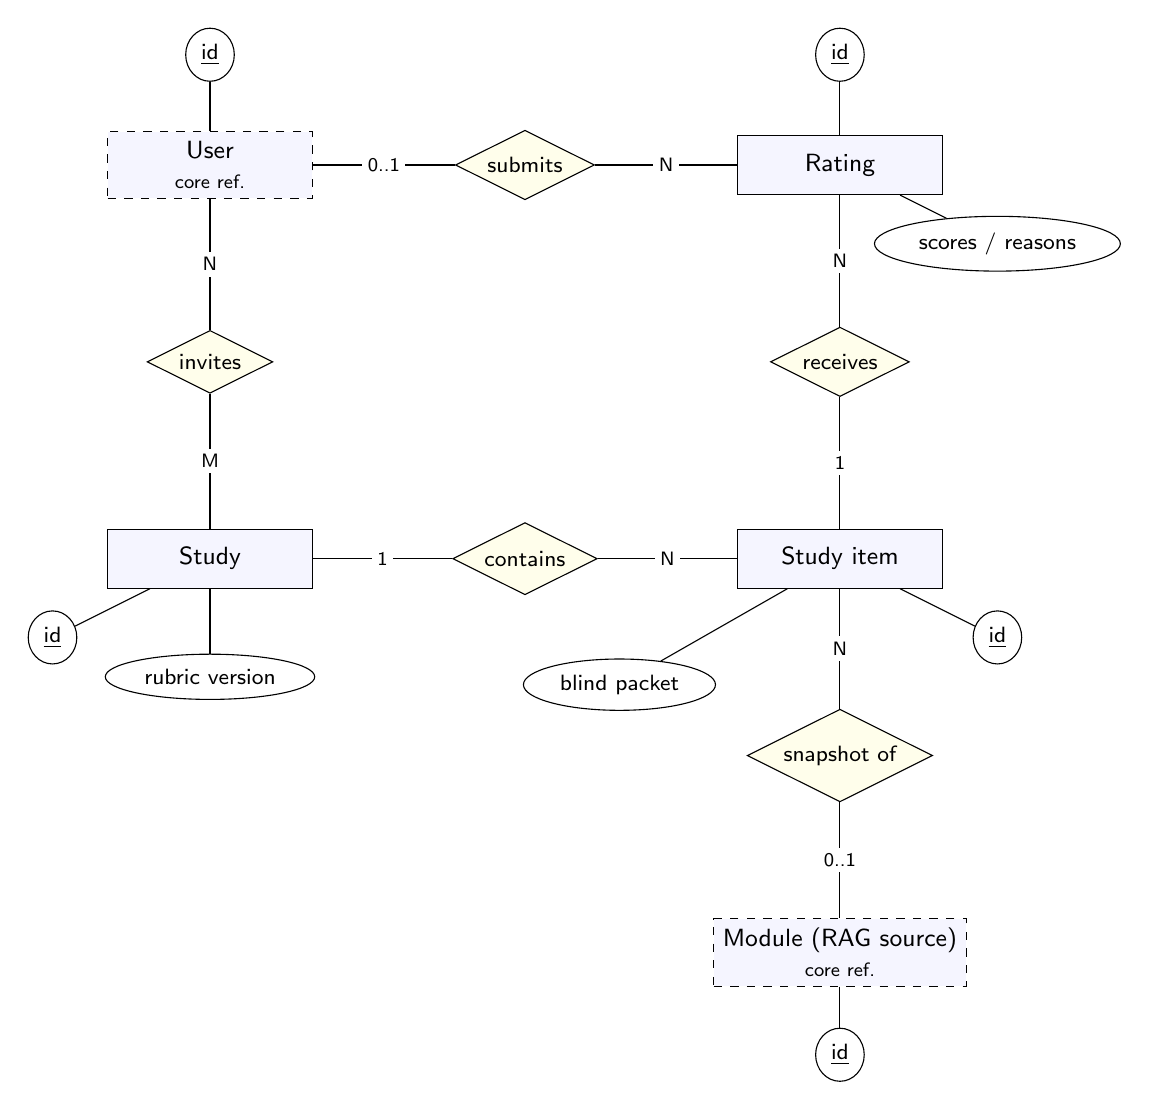
\begin{tikzpicture}[font=\sffamily\small,>=Latex,
box/.style={draw,rounded corners=2pt,align=center,minimum width=3cm,minimum height=1cm,fill=blue!4},
entity/.style={draw,rectangle,align=center,minimum width=2.6cm,minimum height=.75cm,fill=blue!4},
rel/.style={draw,diamond,aspect=2,inner sep=2pt,align=center,font=\sffamily\footnotesize,fill=yellow!8},
attr/.style={draw,ellipse,inner sep=3pt,font=\sffamily\footnotesize},
uc/.style={draw,ellipse,align=center,minimum width=4cm,minimum height=.9cm},
flow/.style={->,thick},lab/.style={font=\sffamily\scriptsize,fill=white,inner sep=2pt}]
\node[entity,dashed] (u) at (0,6) {User\\{\scriptsize core ref.}};
\node[entity] (r) at (8,6) {Rating};
\node[entity] (s) at (0,1) {Study};
\node[entity] (i) at (8,1) {Study item};
\node[entity,dashed] (m) at (8,-4) {Module (RAG source)\\{\scriptsize core ref.}};
\node[rel] (rates) at (4,6) {submits}; \draw (u) -- node[lab]{0..1} (rates); \draw (rates) -- node[lab]{N} (r);
\node[rel] (items) at (4,1) {contains}; \draw (s) -- node[lab]{1} (items); \draw (items) -- node[lab]{N} (i);
\node[rel] (ratings) at (8,3.5) {receives}; \draw (i) -- node[lab]{1} (ratings); \draw (ratings) -- node[lab]{N} (r);
\node[rel] (snap) at (8,-1.5) {snapshot of}; \draw (m) -- node[lab]{0..1} (snap); \draw (snap) -- node[lab]{N} (i);
\node[rel] (invites) at (0,3.5) {invites}; \draw (s) -- node[lab]{M} (invites); \draw (invites) -- node[lab]{N} (u);
\node[attr] (sid) at (-2,0) {\underline{id}}; \draw (s) -- (sid);
\node[attr] (rubric) at (0,-0.5) {rubric version}; \draw (s) -- (rubric);
\node[attr] (iid) at (10,0) {\underline{id}}; \draw (i) -- (iid);
\node[attr] (packet) at (5.2,-0.6) {blind packet}; \draw (i) -- (packet);
\node[attr] (uid) at (0,7.4) {\underline{id}}; \draw (u) -- (uid);
\node[attr] (rid) at (8,7.4) {\underline{id}}; \draw (r) -- (rid);
\node[attr] (score) at (10,5) {scores / reasons}; \draw (r) -- (score);
\node[attr] (mid) at (8,-5.3) {\underline{id}}; \draw (m) -- (mid);
\end{tikzpicture}
\end{document}
